\documentclass[12pt]{article}
\usepackage{amsmath}
\usepackage{graphicx}
\title{Report for Auto Control Lab3 and 4}
\date{2020/9/22}
\author{Jacky Yeh 4107064003}

\begin{document}
\begin{titlepage}

\maketitle
\end{titlepage}


\section{Introduction}
This is the second Experiment of Auto Control Lab where TAs taught us some the use of SIMULINK, a certain block diagram like system flow control interface in MATLAB for us to better understand the use of system flow control and control system plotting.\\

\section{LAB3}
\subsection{Basic usages of SIMULINK and its Interfaces}
Objective:To perform basic operations on SIMULINK.\\
These are the stated Homework problems\\
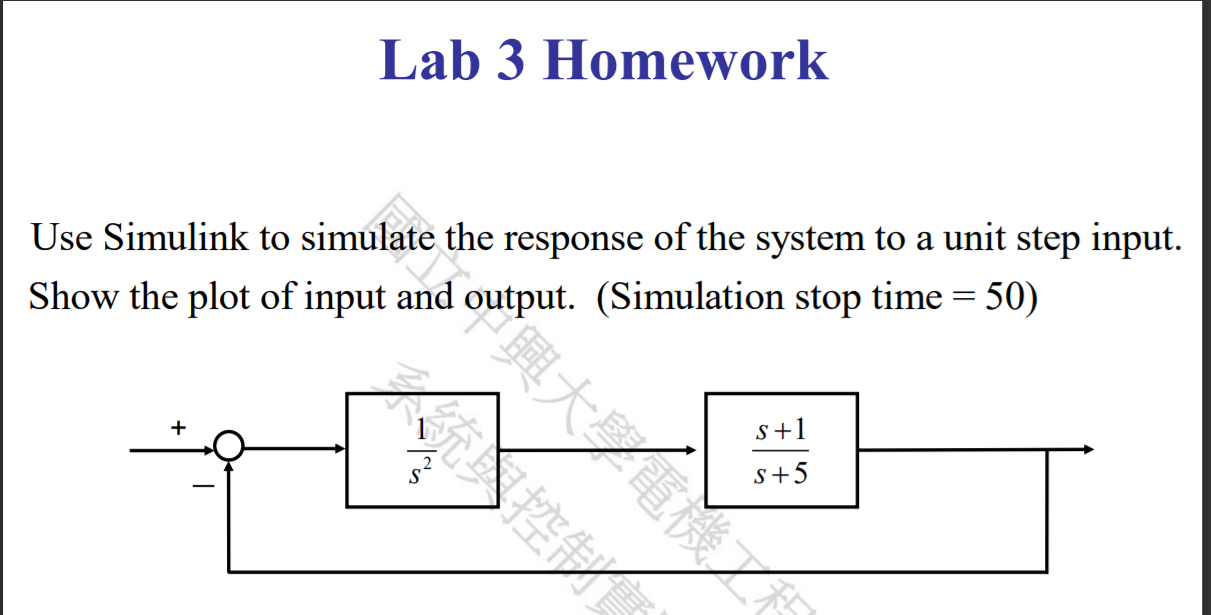
\includegraphics[scale=0.6]{../Lab3,4/HW for lab 3,4/LAB3/LAB3 HW.png}
\cleardoublepage 

\subsection{SIMULINK SYSTEM BLOCK DIAGRAM FOR LAB3}
In order to perform the tasks, SIMULINK flow graph blocks are needed.The following is the control flow graph for SIMULINK\\

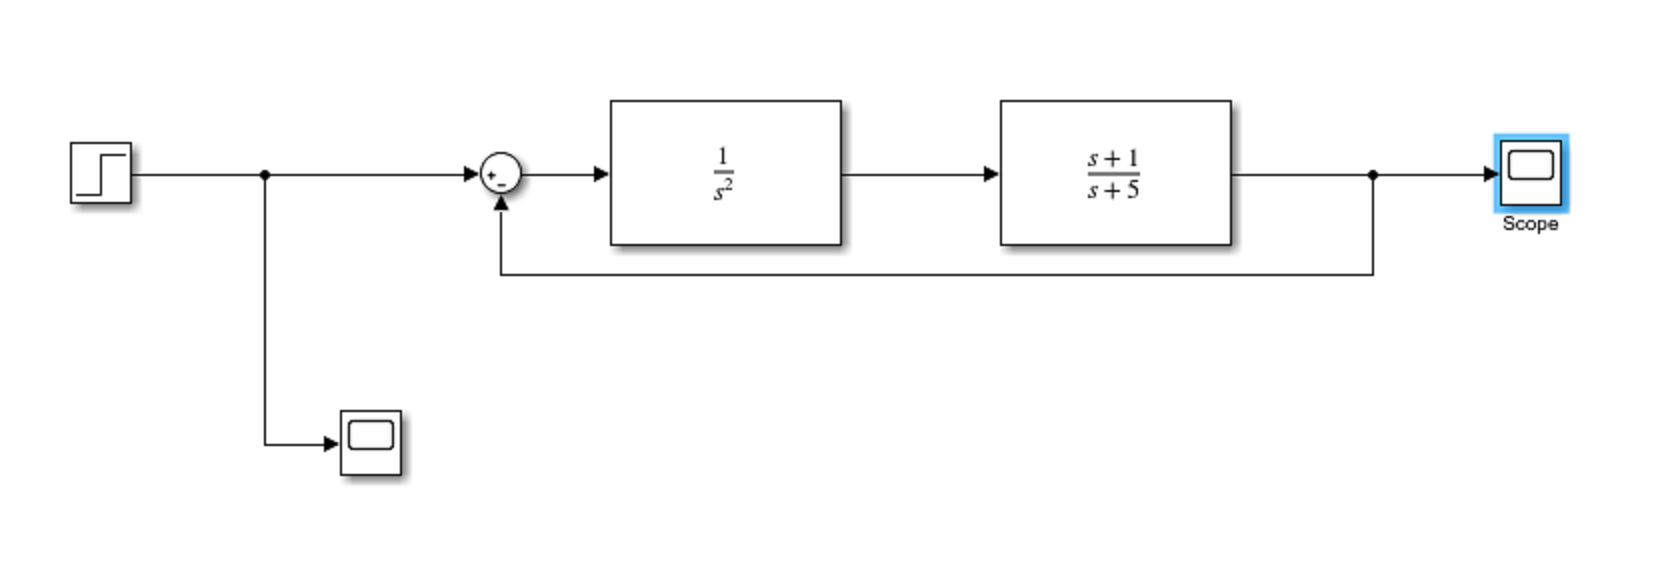
\includegraphics[scale=0.5]{../Lab3,4/HW for lab 3,4/LAB3/Block_diagram.png} 
\\
\cleardoublepage
\subsection{Results of SIMULINK PLOT} 
The results contains of Input and output, where input is a unit step function and output is the plot of this certain transfer function for this system\\

\begin{center}
Input of the unit step function$$u(t),\forall t>=0$$\\
\end{center}
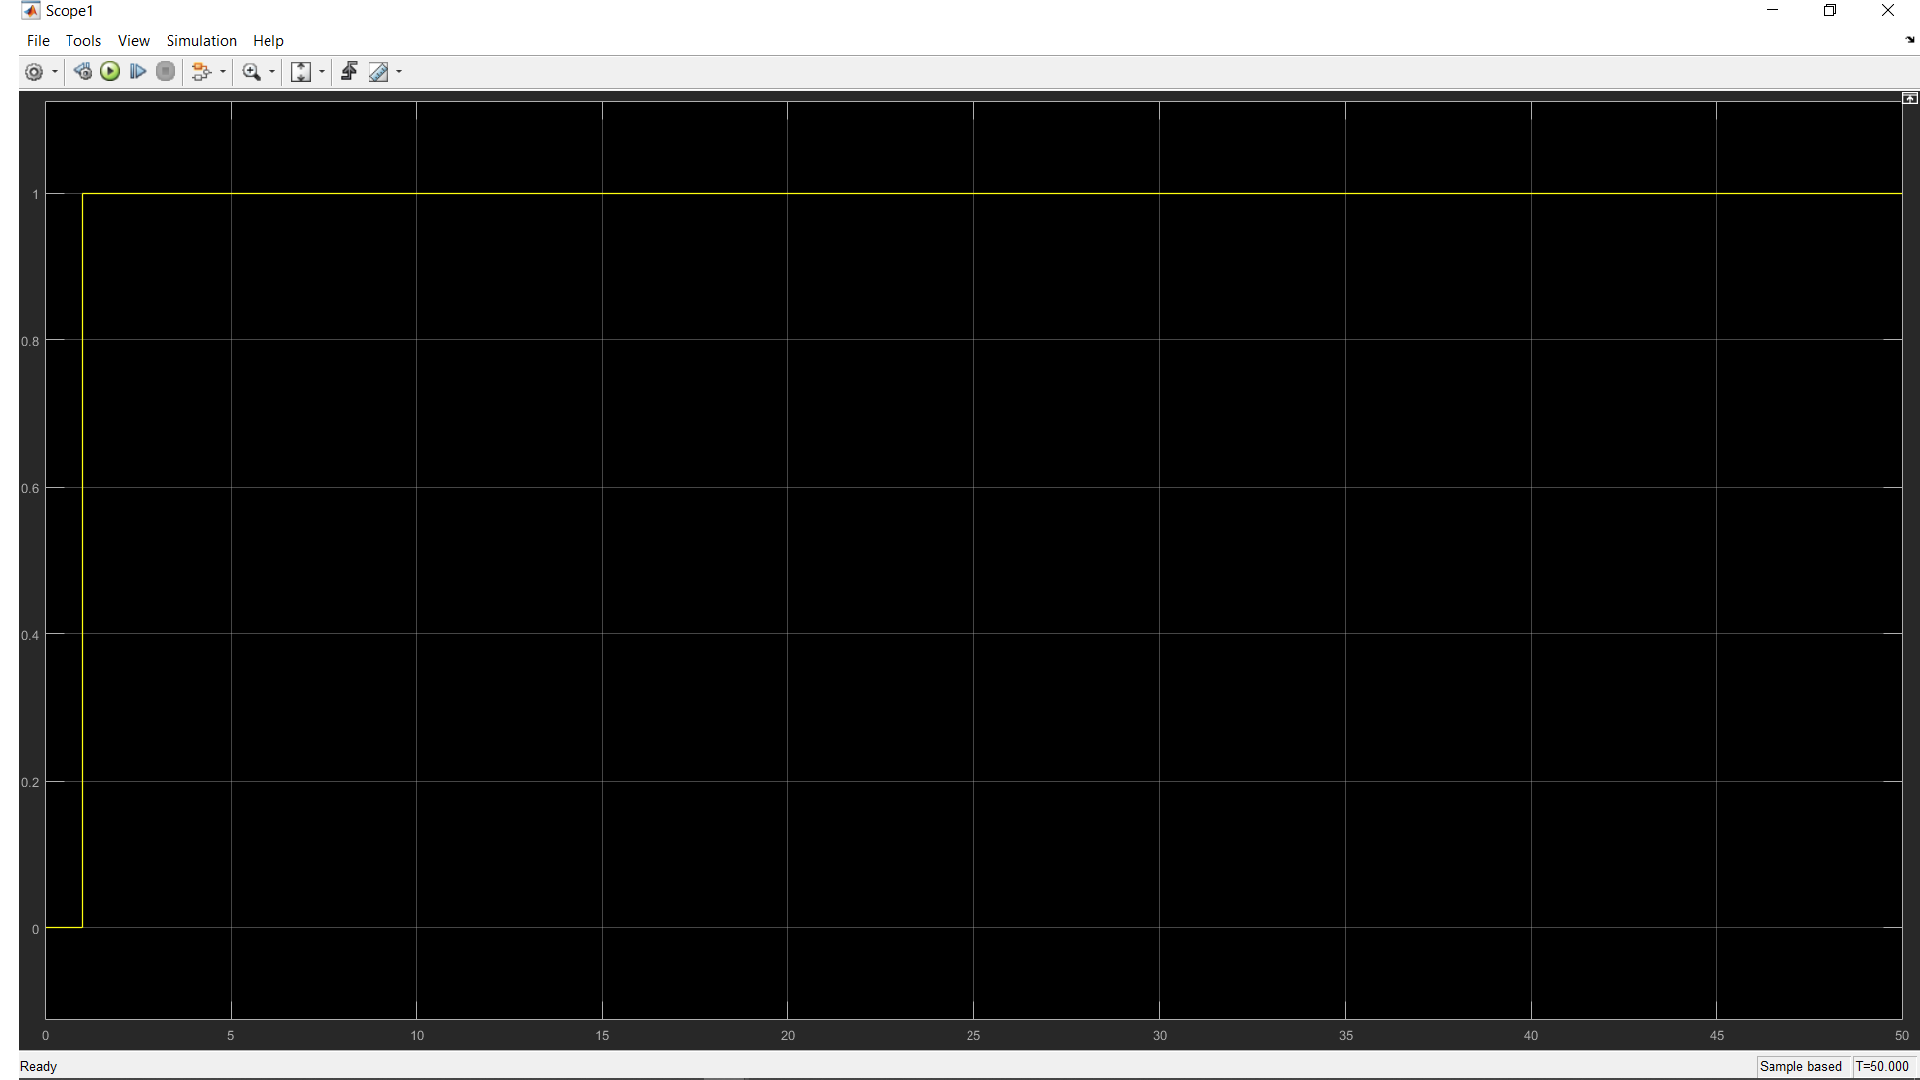
\includegraphics[scale=0.4]{../Lab3,4/HW for lab 3,4/LAB3/Input.png}\\

\cleardoublepage 

\begin{center}
Output of this in MATLAB AND SCOPE for this complex SYSTEM\\
\end{center}
 
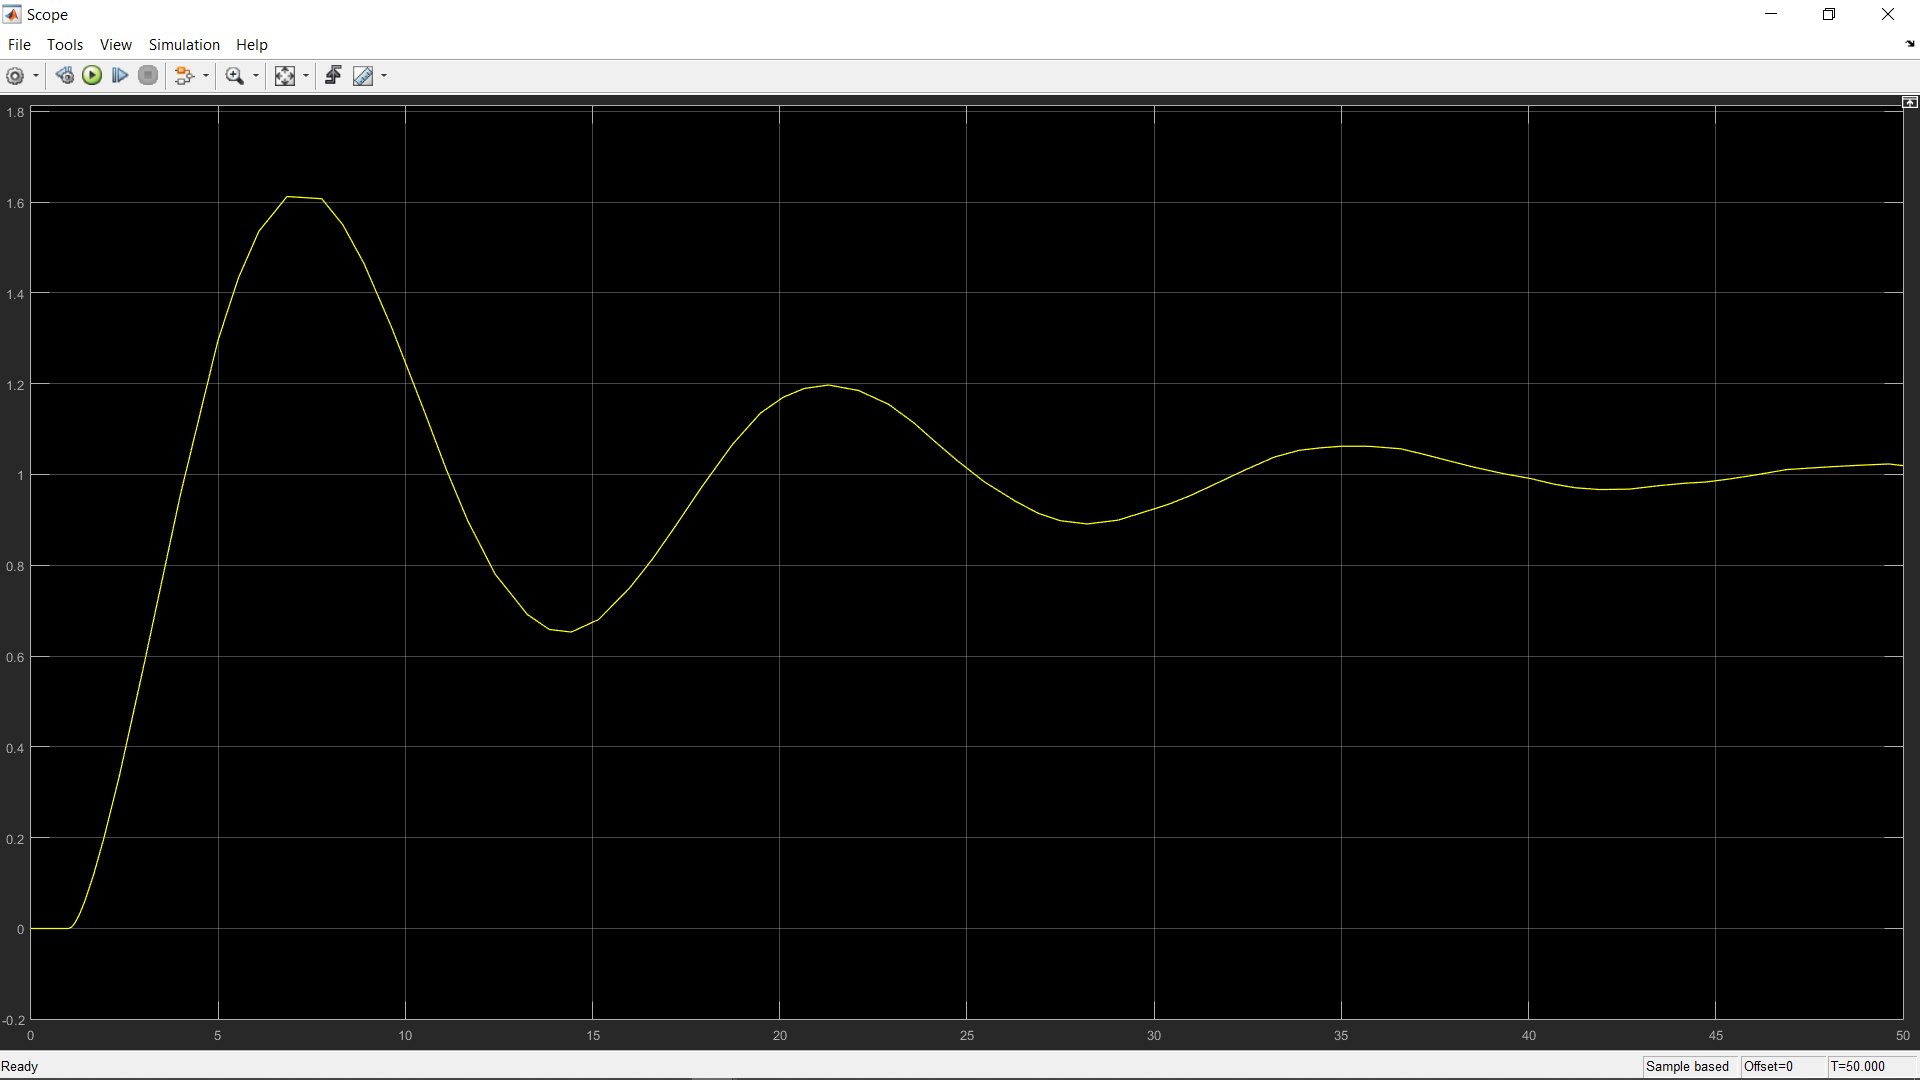
\includegraphics[scale=0.4]{../Lab3,4/HW for lab 3,4/LAB3/Scope.png}\\
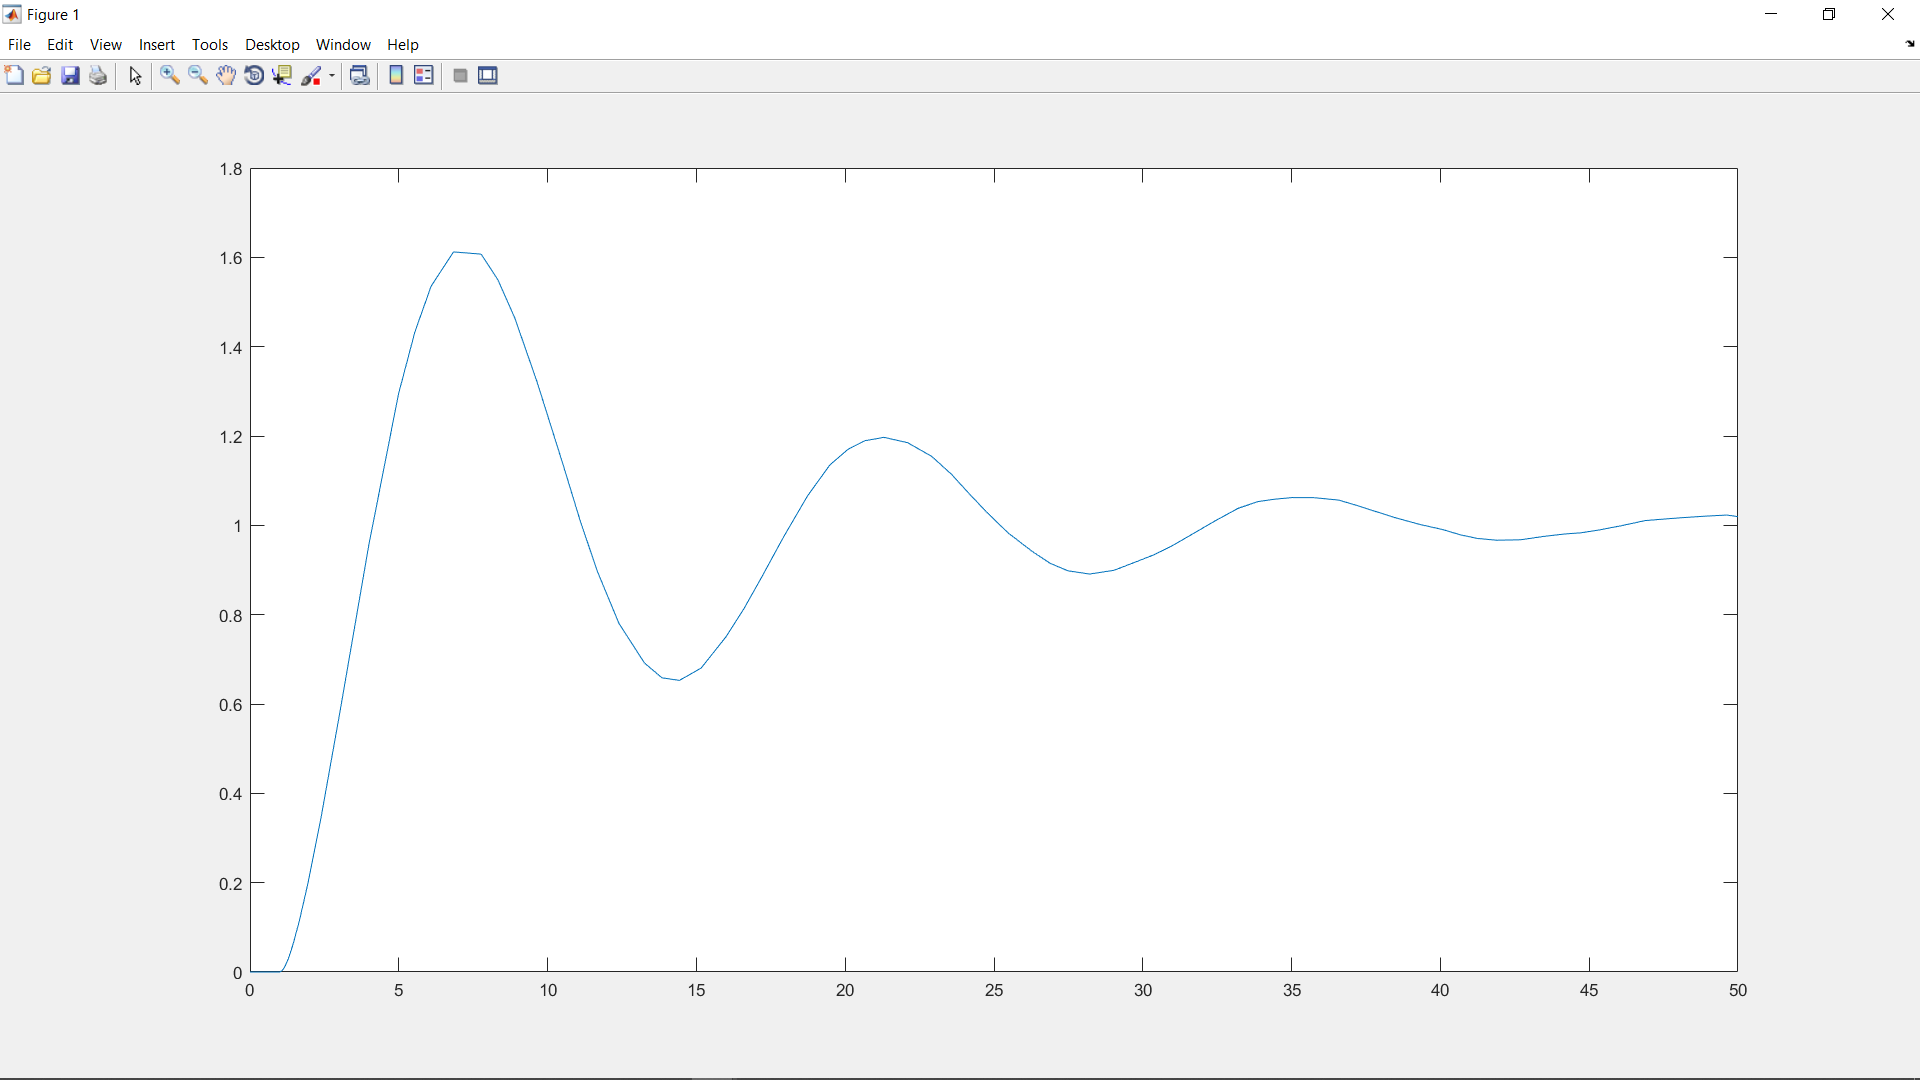
\includegraphics[scale=0.4]{../Lab3,4/HW for lab 3,4/LAB3/Plot.png}  


\section{LAB4}
\subsection{More basic usages with SIMULINK, the graph of PID controller system}
Objective:To perform more basic functions on Simulink and some introduction on PID controller, and its influence on the system with P, PI and PID controller block diagram involved\\
\\
\begin{center}
HW for LAB4\\
\end{center}

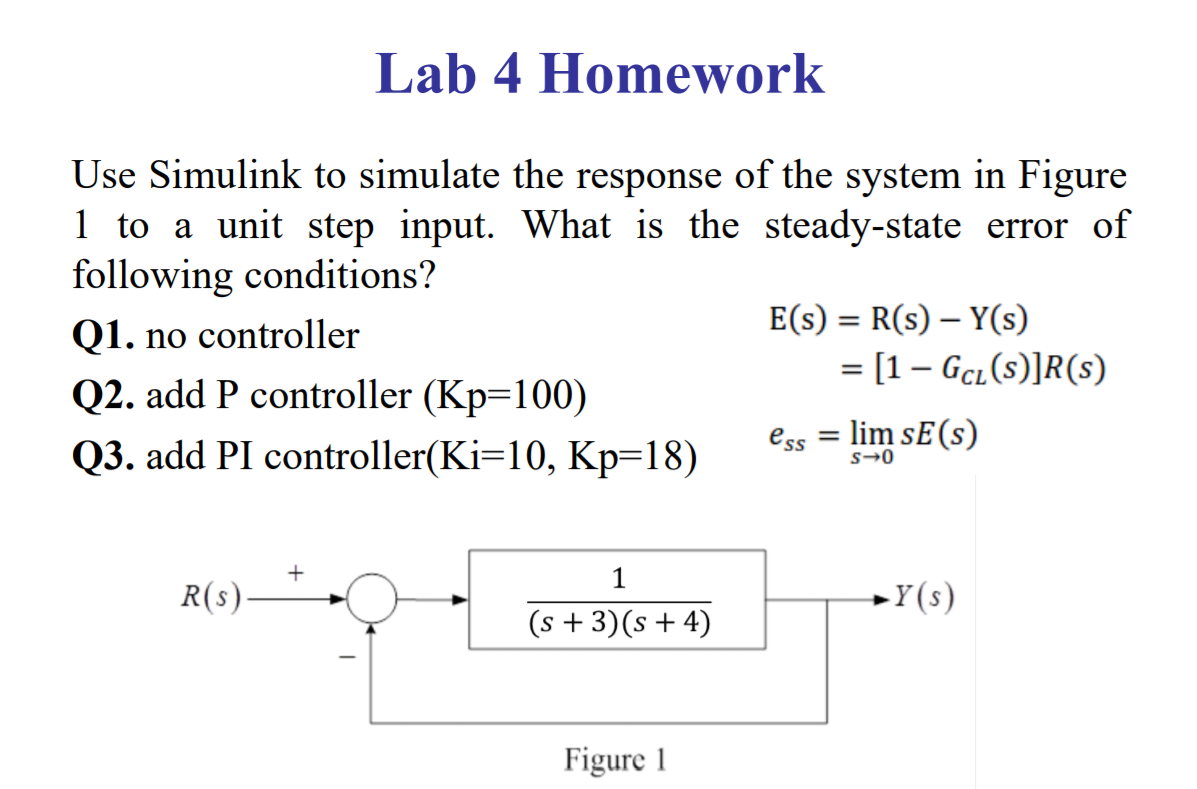
\includegraphics[scale=0.6]{../Lab3,4/HW for lab 3,4/LAB4/LAB4 HW.png}
\cleardoublepage  

\subsection{SIMULINK BLOCK DIAGRAM for Lab4}
\subparagraph{Problem 1,System with no PID control and its  error function plot}
\begin{center}
The block diagram in SIMULINK for problem 1\\
\end{center}
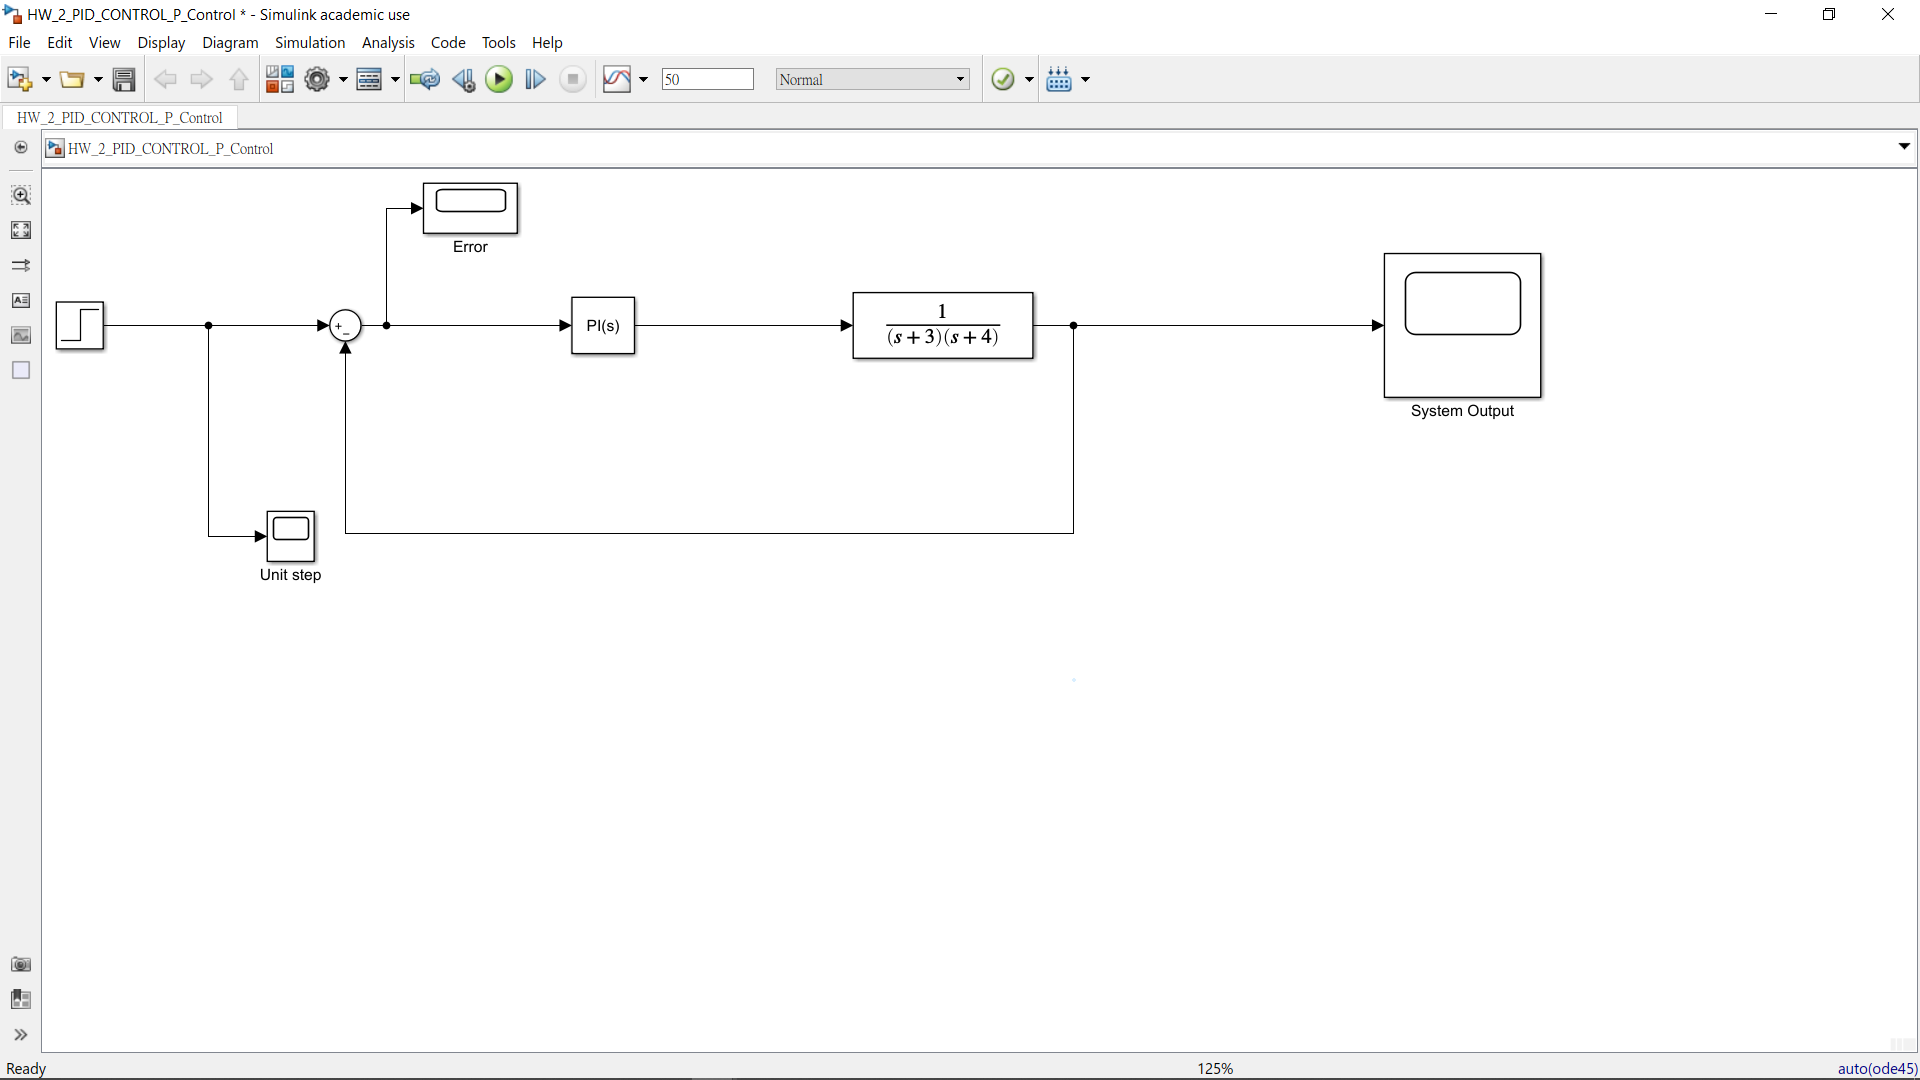
\includegraphics[scale=0.3]{../Lab3,4/HW for lab 3,4/LAB4/Block_diagram_PID_controller.png}\\ 



Input of the unit step function$$u(t),\forall t>=0$$\\
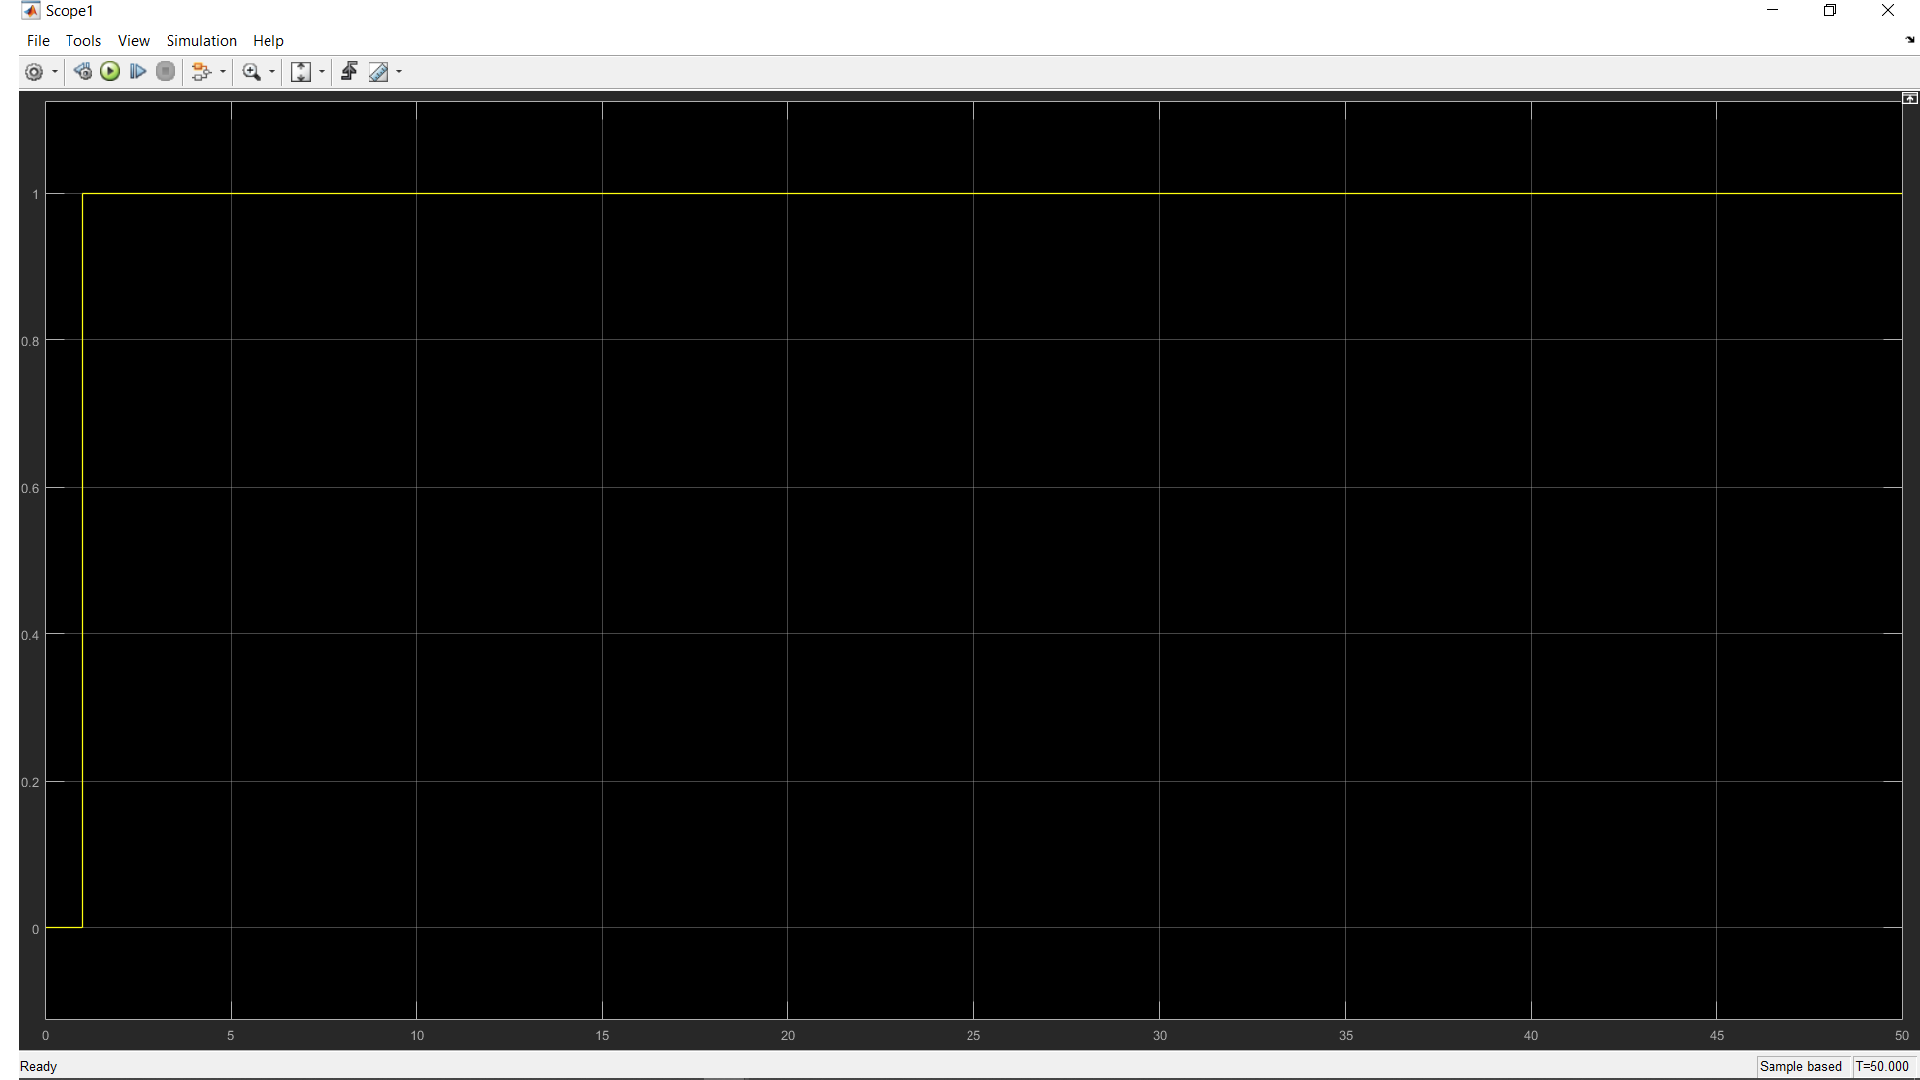
\includegraphics[scale=0.3]{../Lab3,4/HW for lab 3,4/LAB3/Input.png}\\

\begin{center}
The computed results and Error function are shown below for problem 1\\
\end{center}
  
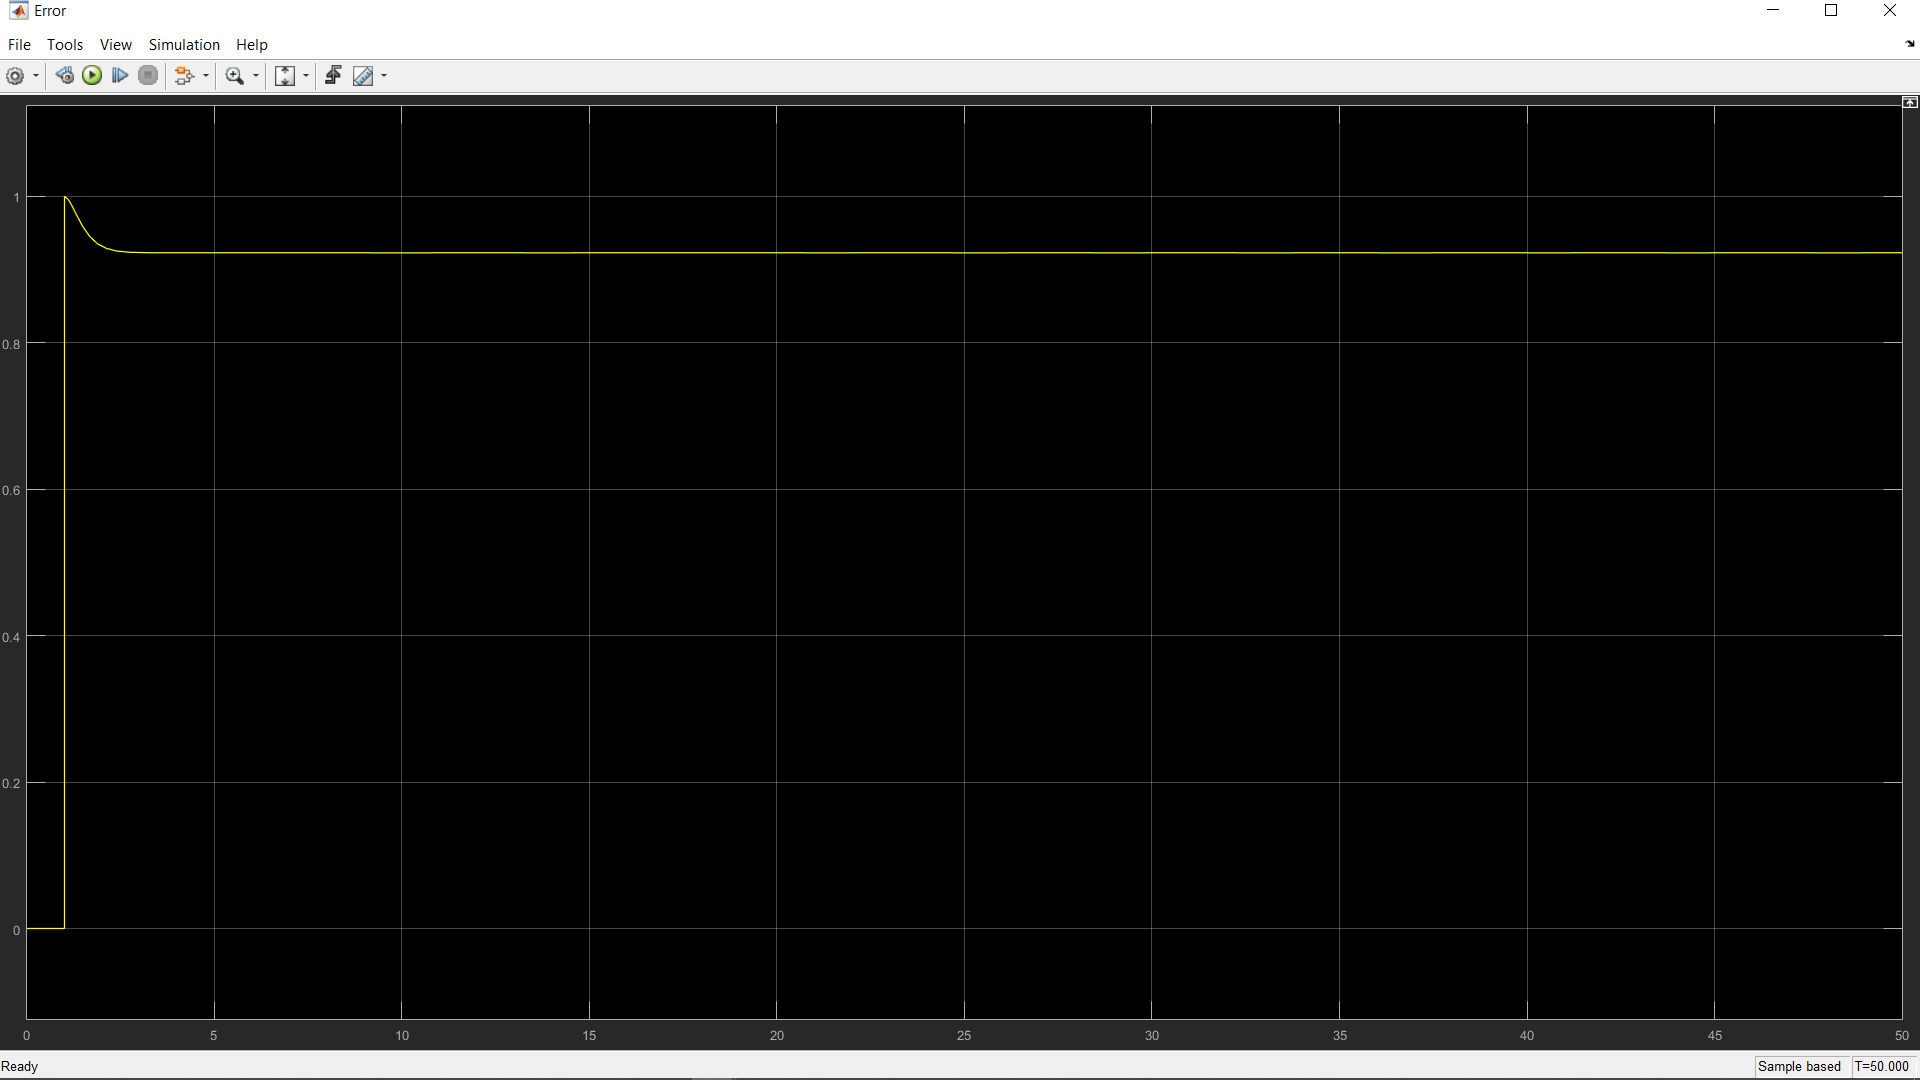
\includegraphics[scale=0.4]{../Lab3,4/HW for lab 3,4/LAB4/Error_1_No_controller.png}\\
\cleardoublepage
\subparagraph{Problem 2, system with P controller}
\begin{center}
The computed results and Error function are shown below for problem 2\\
\end{center}

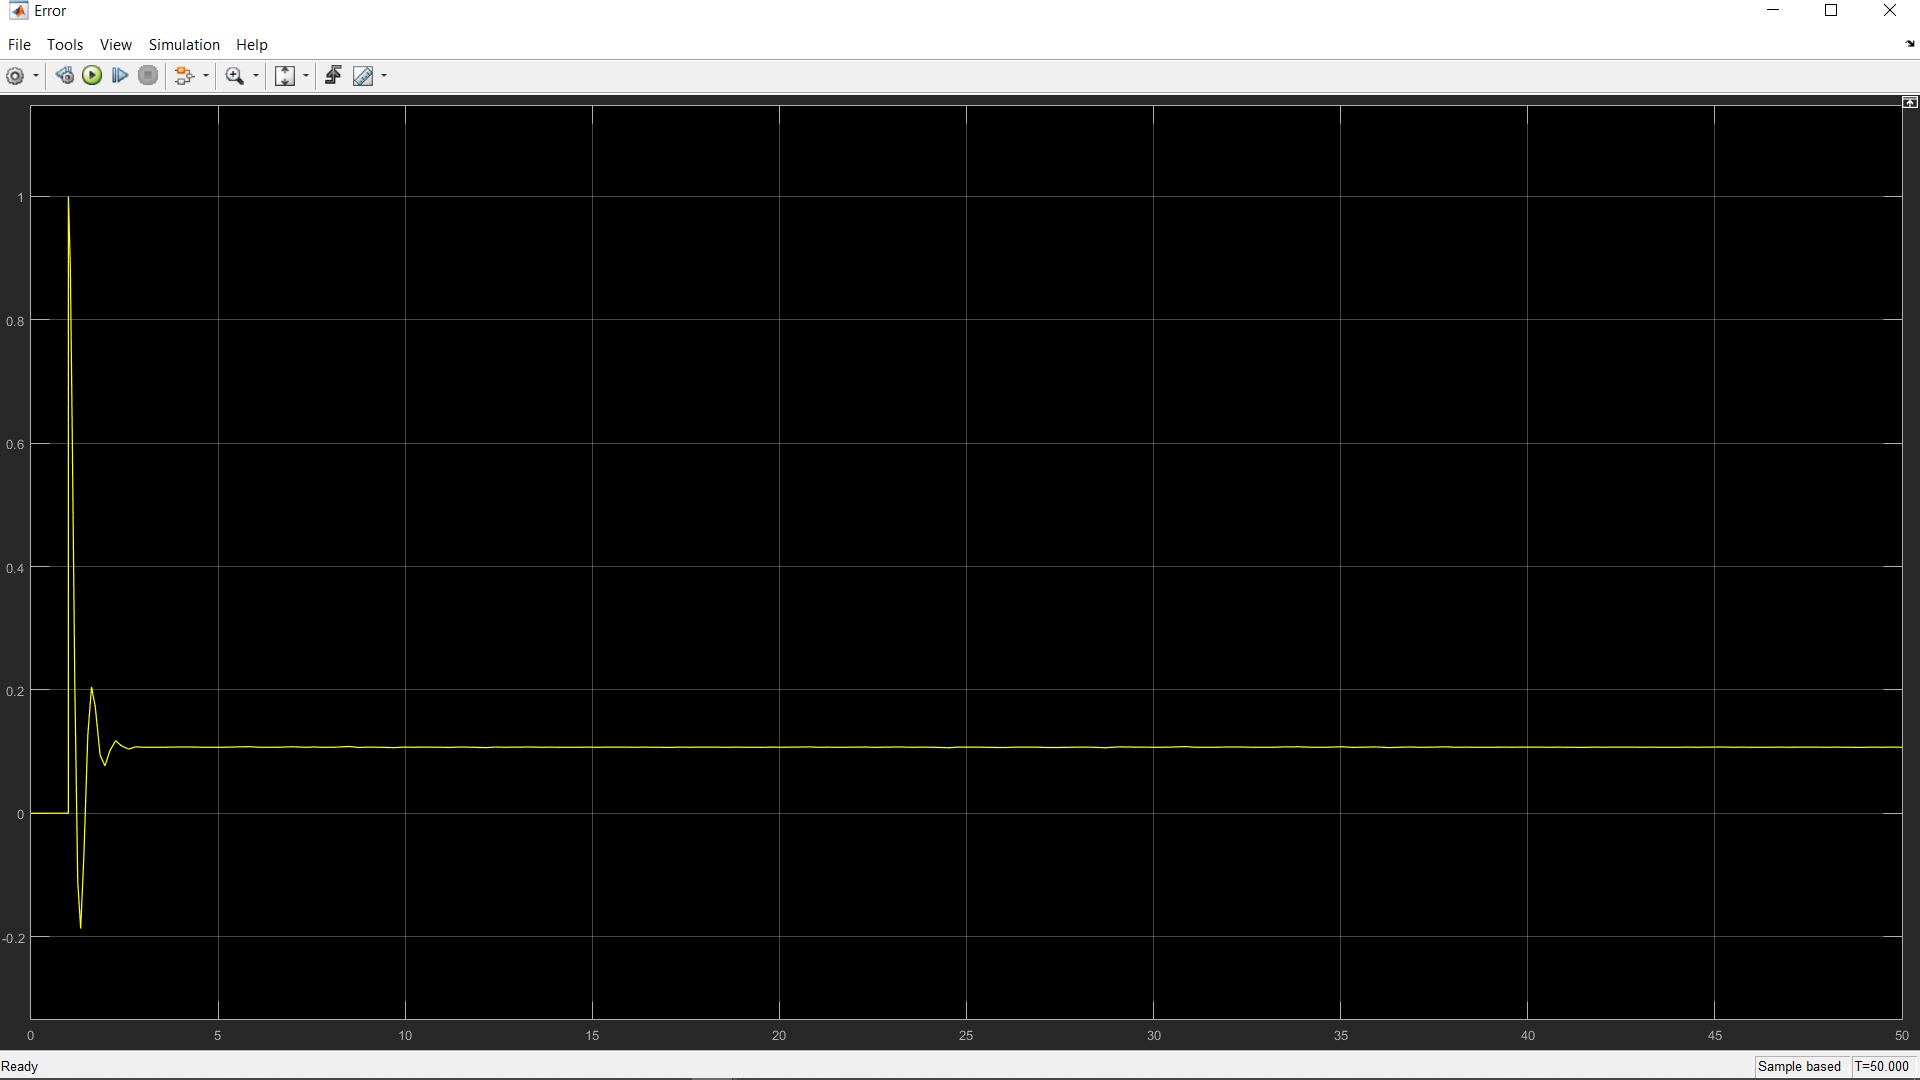
\includegraphics[scale=0.3]{../Lab3,4/HW for lab 3,4/LAB4/Error_2_P_controller.png} \\
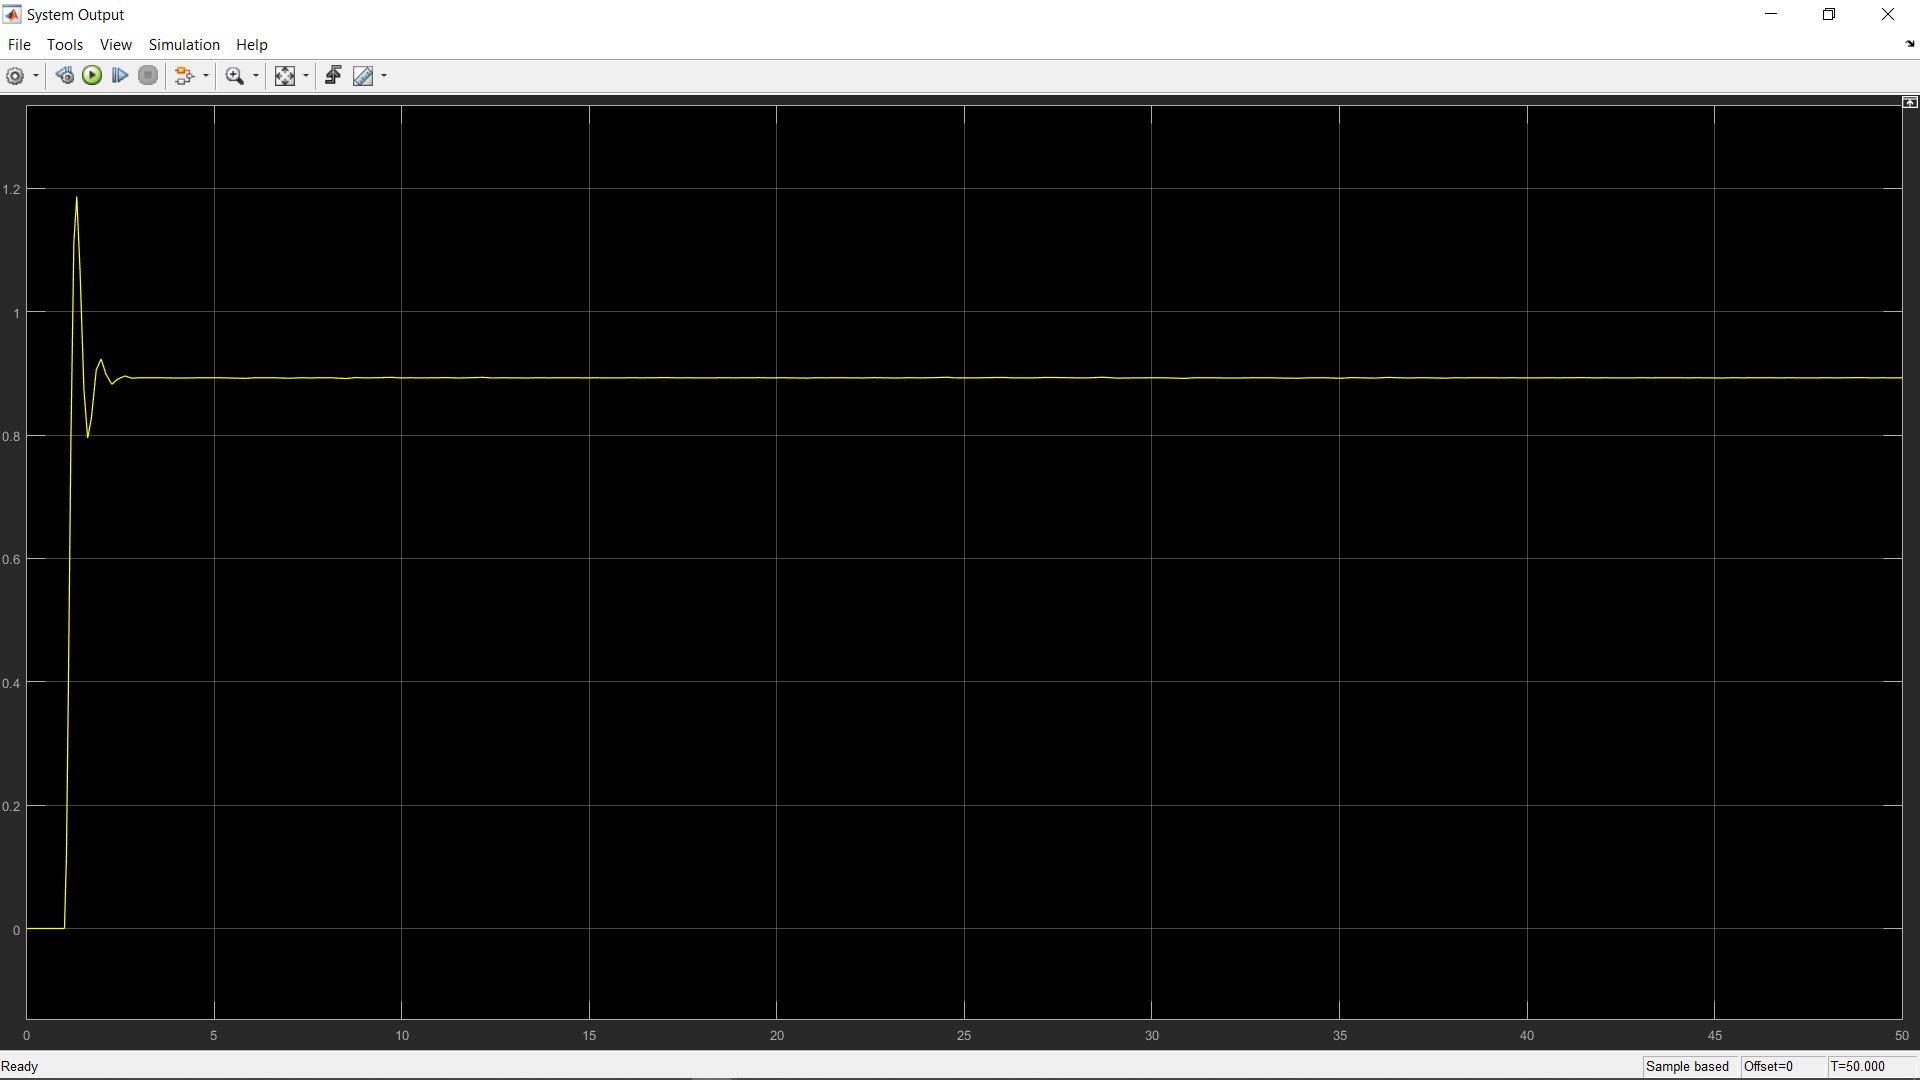
\includegraphics[scale=0.3]{../Lab3,4/HW for lab 3,4/LAB4/OUTPUT_2_P_controller.png} \\

\cleardoublepage
\subparagraph{Problem 3, system with PI controller}
\begin{center}
The computed results and Error function are shown below for problem 3\\
\end{center}

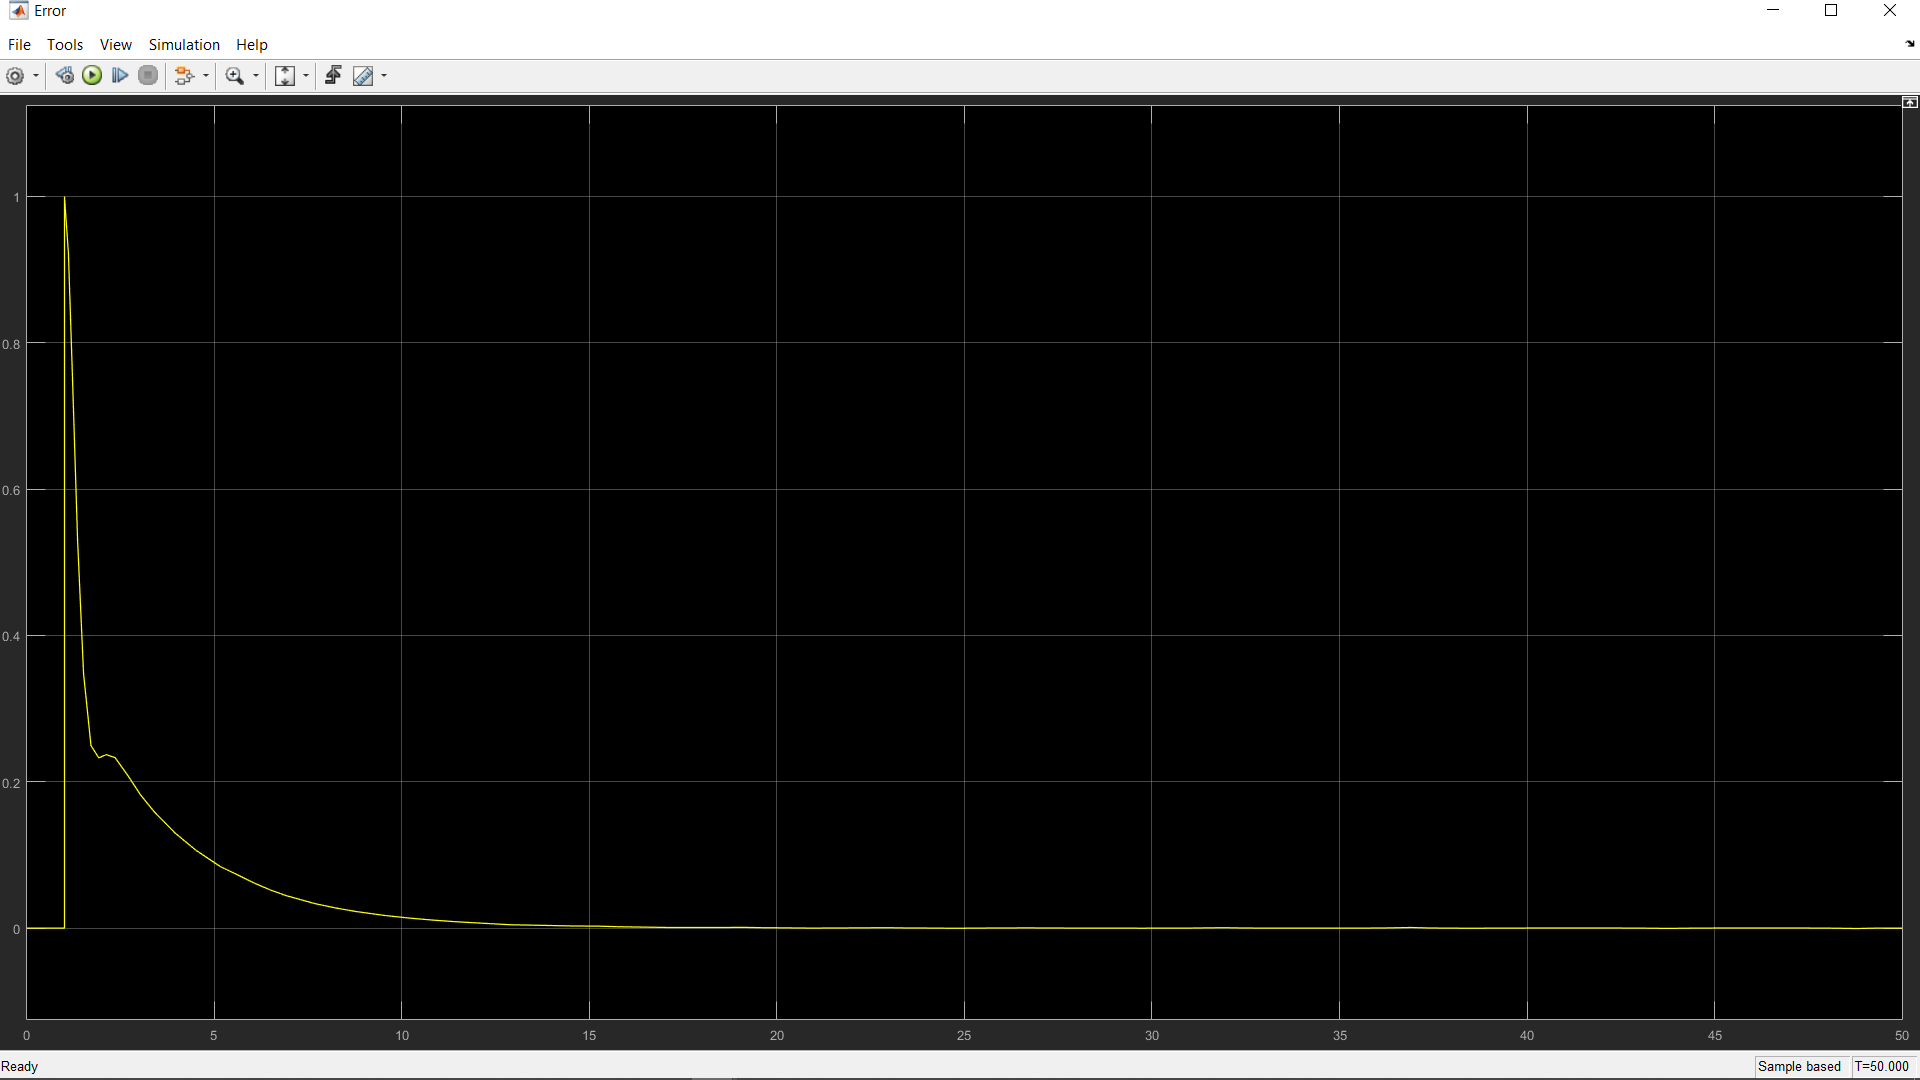
\includegraphics[scale=0.3]{../Lab3,4/HW for lab 3,4/LAB4/ERROR_3_PI_controller.png}\\ 
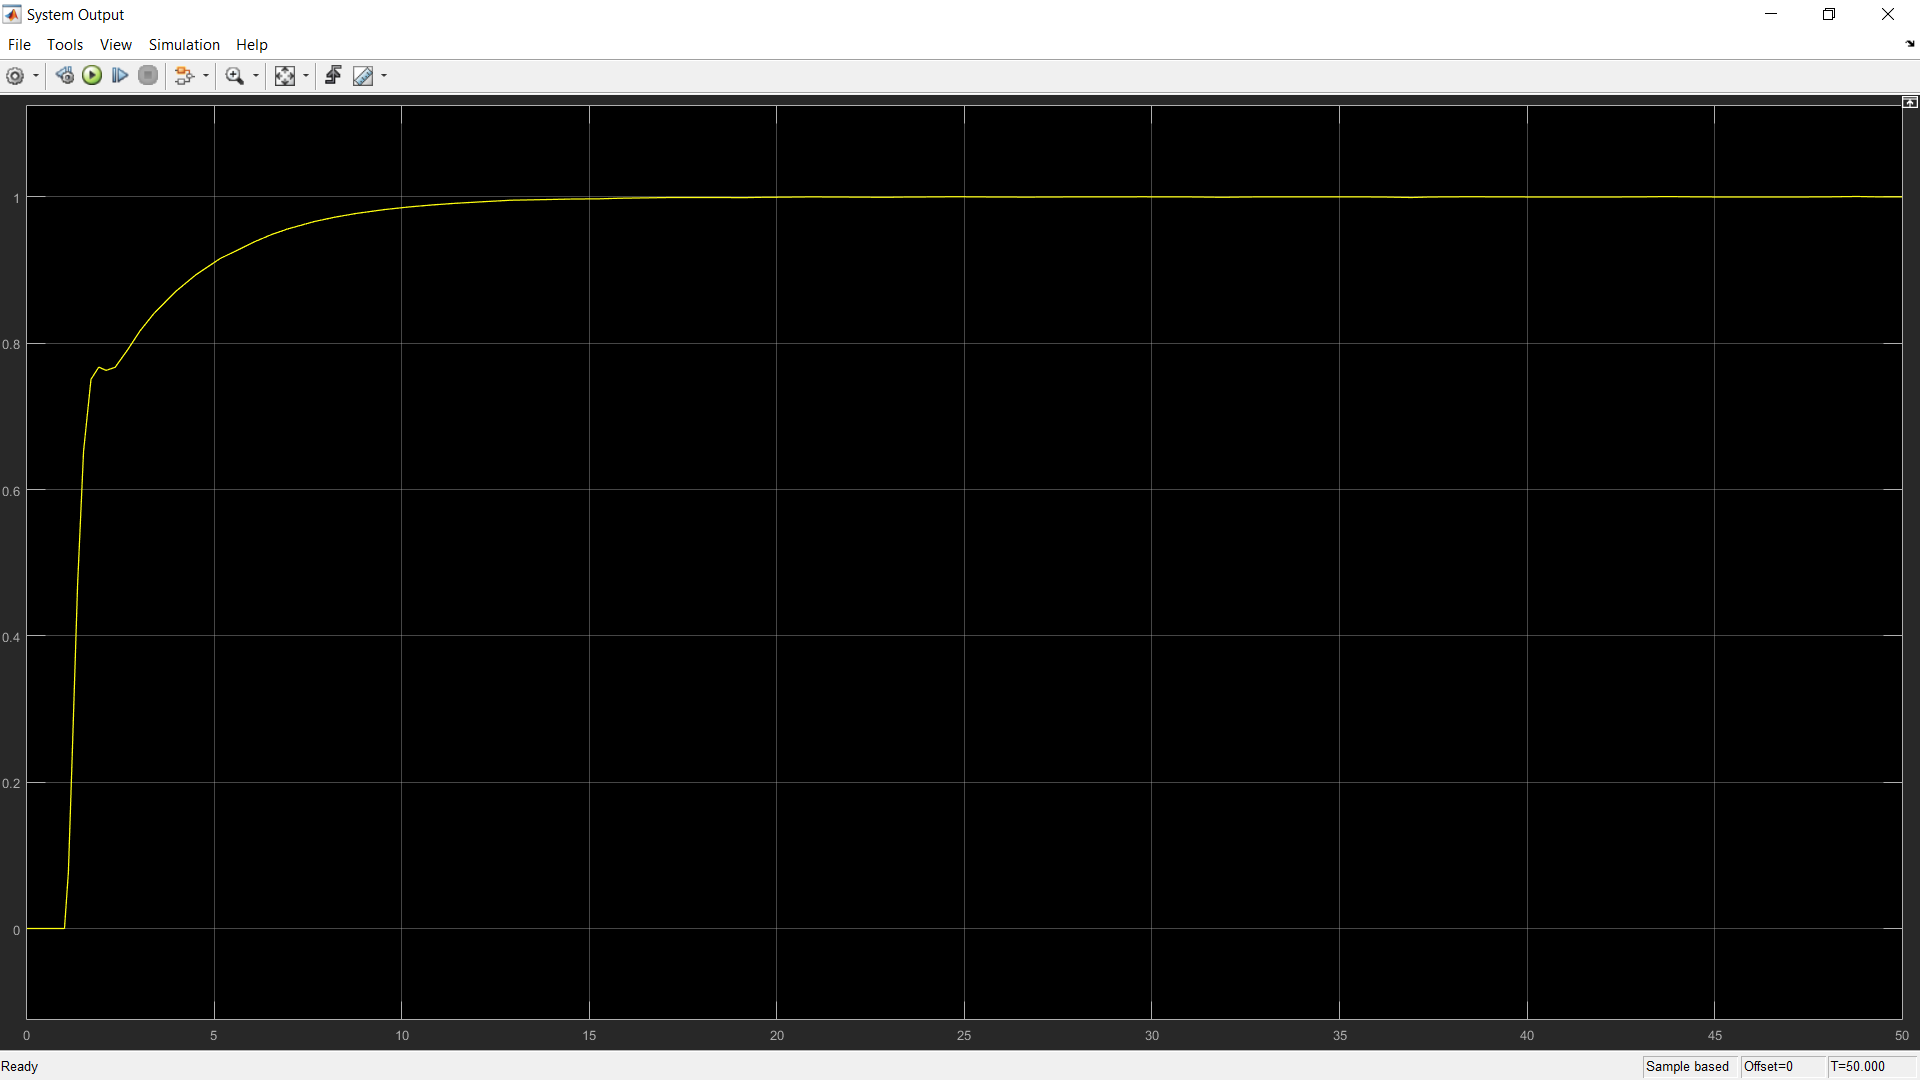
\includegraphics[scale=0.3]{../Lab3,4/HW for lab 3,4/LAB4/OUTPUT_3_PI_controller.png}\\ 
\cleardoublepage


\section{Conclusion}
This is the second Lab for auto control , today TAs teach us how to ultilize the powerful usages of MATLAB in SIMULINK block interface. Which makes visualise control flow system an easy task. As always, these usages in plotting graph and observing system output and building systems shall be trained as an intuition for further course in MATLAB programming, otherwise without the knowledge with these operations, you might have problems in dealing with even more complex system\\
\begin{center} 
This concludes the second Week of Auto Control LAB\\
\end{center}

\end{document} 
